\documentclass[12pt,a4paper]{article}
\usepackage{tikz}
\usepackage{pgfplots}
\usepackage{pgf-pie}
\usetikzlibrary{shapes.geometric, shapes.multipart, arrows.meta, positioning, fit, calc, backgrounds}
\pgfplotsset{compat=1.18}

\begin{document}

% ==============================================================================
% DIAGRAM 1: UML USE CASE DIAGRAM
% Useful for Chapter 3: System Design / Requirement Analysis
% Shows how the Farmer and Cloud interact with the system modules.
% ==============================================================================
\section*{1. UML Use Case Diagram}

\begin{figure}[htbp]
\centering
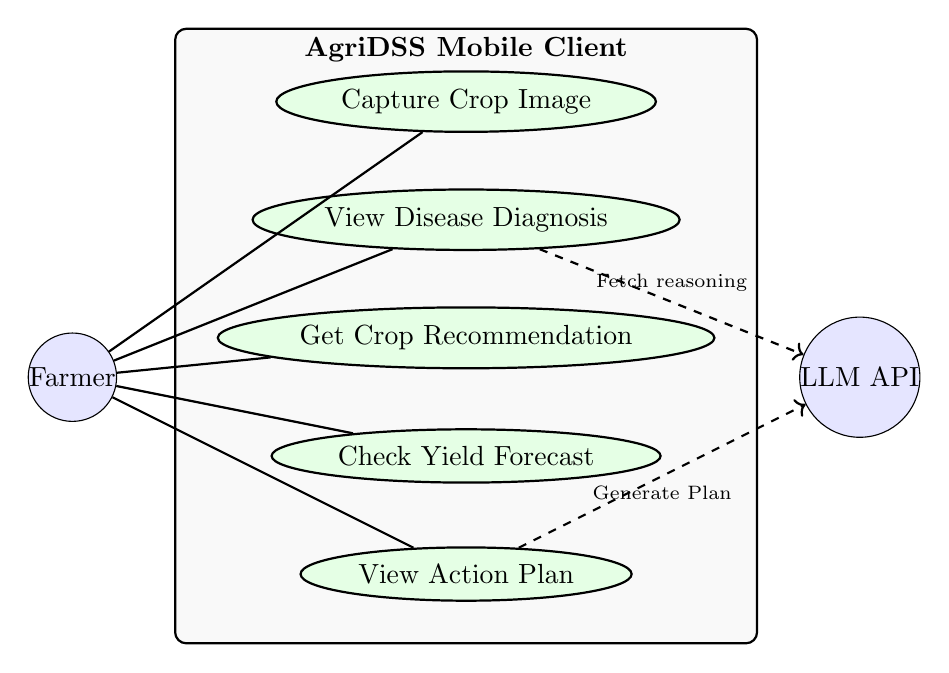
\begin{tikzpicture}[
  actor/.style={circle, draw, minimum size=1cm, inner sep=0pt, fill=blue!10},
  usecase/.style={ellipse, draw, thick, fill=green!10, minimum width=3cm, align=center},
  line/.style={draw, thick, -}
]

% Actors
\node[actor] (farmer) at (0, 0) {Farmer};
\node[actor] (cloud) at (10, 0) {LLM API};

% Use Cases
\node[usecase] (uc1) at (5, 3.5) {Capture Crop Image};
\node[usecase] (uc2) at (5, 2) {View Disease Diagnosis};
\node[usecase] (uc3) at (5, 0.5) {Get Crop Recommendation};
\node[usecase] (uc4) at (5, -1) {Check Yield Forecast};
\node[usecase] (uc5) at (5, -2.5) {View Action Plan};

% System Boundary
\begin{pgfonlayer}{background}
  \node[draw, thick, rounded corners, fill=gray!5, fit=(uc1) (uc2) (uc3) (uc4) (uc5), inner sep=15pt, label={[font=\bfseries, anchor=north]above:AgriDSS Mobile Client}] (sys) {};
\end{pgfonlayer}

% Connections
\draw[line] (farmer) -- (uc1);
\draw[line] (farmer) -- (uc2);
\draw[line] (farmer) -- (uc3);
\draw[line] (farmer) -- (uc4);
\draw[line] (farmer) -- (uc5);

\draw[line, dashed, ->] (uc2) -- (cloud) node[midway, above, font=\scriptsize] {Fetch reasoning};
\draw[line, dashed, ->] (uc5) -- (cloud) node[midway, below, font=\scriptsize] {Generate Plan};

\end{tikzpicture}
\caption{UML Use Case Diagram showing farmer interactions with the AgriDSS platform.}
\end{figure}

\vspace{1cm}

% ==============================================================================
% DIAGRAM 2: DETAILED MODULE SEQUENCE DIAGRAM
% Useful for Chapter 4 or 5: Shows the exact flow of data over time
% ==============================================================================
\section*{2. Sequence Diagram (Disease Detection \& Reasoning)}

\begin{figure}[htbp]
\centering
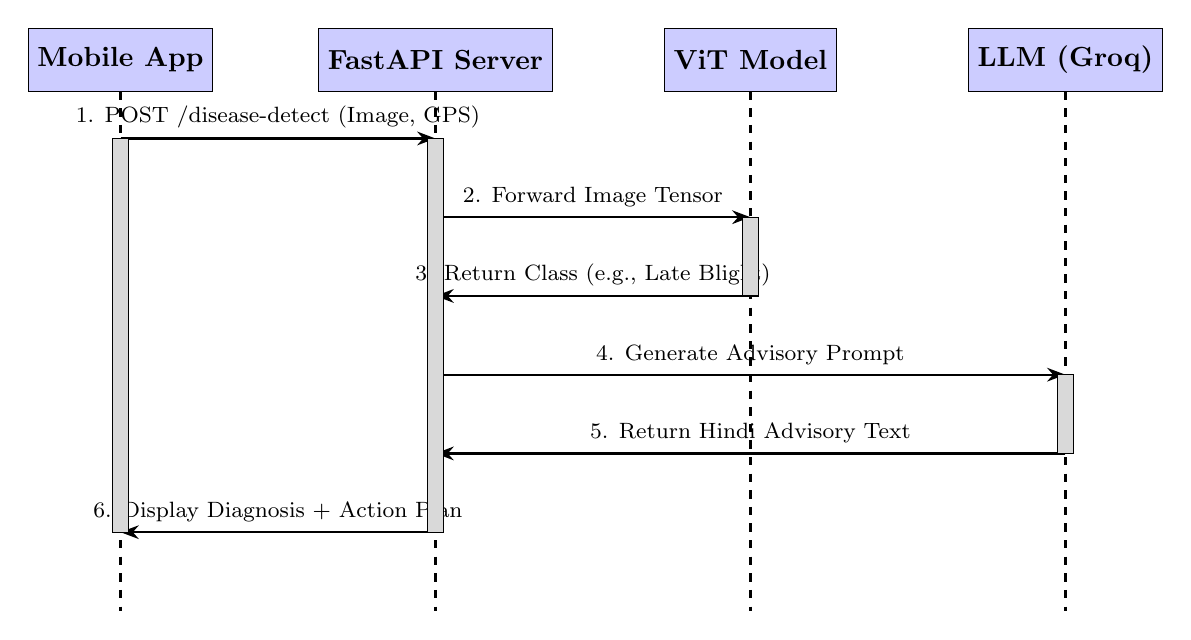
\begin{tikzpicture}[
  node distance=2cm,
  auto,
  lifeline/.style={thick, dashed},
  box/.style={rectangle, draw, fill=blue!20, minimum width=2cm, minimum height=0.8cm, font=\bfseries}
]

% Participants
\node[box] (app) at (0,0) {Mobile App};
\node[box] (api) at (4,0) {FastAPI Server};
\node[box] (vit) at (8,0) {ViT Model};
\node[box] (llm) at (12,0) {LLM (Groq)};

% Lifelines
\draw[lifeline] (app) -- (0,-7);
\draw[lifeline] (api) -- (4,-7);
\draw[lifeline] (vit) -- (8,-7);
\draw[lifeline] (llm) -- (12,-7);

% Messages
\draw[-{Stealth}, thick] (0,-1) -- (4,-1) node[midway, above, font=\footnotesize] {1. POST /disease-detect (Image, GPS)};
\draw[-{Stealth}, thick] (4,-2) -- (8,-2) node[midway, above, font=\footnotesize] {2. Forward Image Tensor};
\draw[-{Stealth}, thick] (8,-3) -- (4,-3) node[midway, above, font=\footnotesize] {3. Return Class (e.g., Late Blight)};
\draw[-{Stealth}, thick] (4,-4) -- (12,-4) node[midway, above, font=\footnotesize] {4. Generate Advisory Prompt};
\draw[-{Stealth}, thick] (12,-5) -- (4,-5) node[midway, above, font=\footnotesize] {5. Return Hindi Advisory Text};
\draw[-{Stealth}, thick] (4,-6) -- (0,-6) node[midway, above, font=\footnotesize] {6. Display Diagnosis + Action Plan};

% Execution Bars (Optional visualization)
\filldraw[fill=gray!30] (-0.1,-1) rectangle (0.1,-6);
\filldraw[fill=gray!30] (3.9,-1) rectangle (4.1,-6);
\filldraw[fill=gray!30] (7.9,-2) rectangle (8.1,-3);
\filldraw[fill=gray!30] (11.9,-4) rectangle (12.1,-5);

\end{tikzpicture}
\caption{Sequence diagram detailing the API interaction for the plant disease detection and advisory module.}
\end{figure}

\newpage

% ==============================================================================
% DIAGRAM 3: STATE TRANSITION DIAGRAM
% Useful for Chapter 3: Offline Architecture / Graceful Degradation
% ==============================================================================
\section*{3. State Transition Diagram (Connectivity Engine)}

\begin{figure}[htbp]
\centering
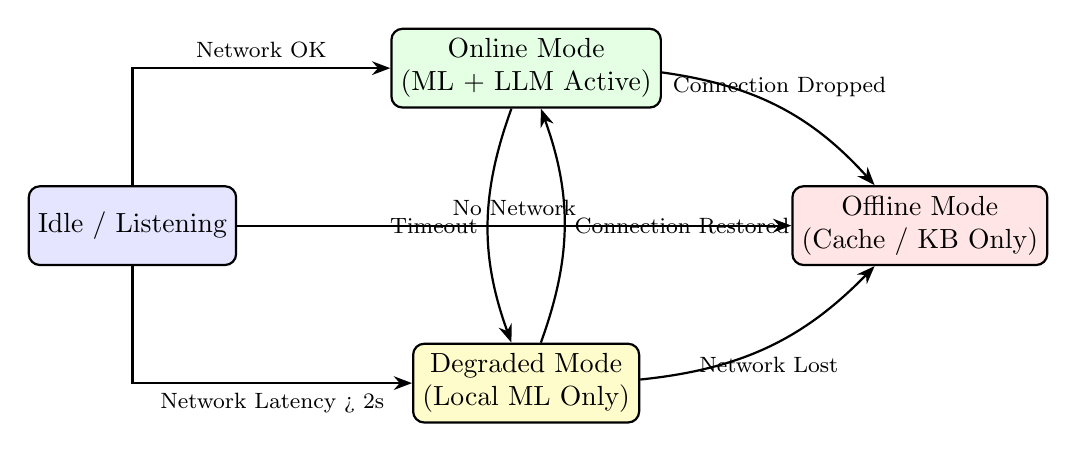
\begin{tikzpicture}[
  state/.style={rectangle, rounded corners, draw, thick, fill=blue!10, minimum width=2.5cm, minimum height=1cm, align=center},
  arr/.style={->, -{Stealth}, thick}
]

\node[state] (idle) at (0, 0) {Idle / Listening};
\node[state, fill=green!10] (online) at (5, 2) {Online Mode\\(ML + LLM Active)};
\node[state, fill=yellow!20] (degraded) at (5, -2) {Degraded Mode\\(Local ML Only)};
\node[state, fill=red!10] (offline) at (10, 0) {Offline Mode\\(Cache / KB Only)};

\draw[arr] (idle) |- node[pos=0.75, above, font=\footnotesize] {Network OK} (online);
\draw[arr] (idle) |- node[pos=0.75, below, font=\footnotesize] {Network Latency > 2s} (degraded);
\draw[arr] (idle) -- node[above, font=\footnotesize] {No Network} (offline);

\draw[arr] (online) edge[bend right=20] node[left, font=\footnotesize] {Timeout} (degraded);
\draw[arr] (degraded) edge[bend right=20] node[right, font=\footnotesize] {Connection Restored} (online);

\draw[arr] (degraded) edge[bend right=20] node[below, font=\footnotesize] {Network Lost} (offline);
\draw[arr] (online) edge[bend left=20] node[above, font=\footnotesize] {Connection Dropped} (offline);

\end{tikzpicture}
\caption{State transition diagram illustrating the graceful degradation logic in the mobile application.}
\end{figure}

\vspace{1cm}

% ==============================================================================
% DIAGRAM 4: MODEL ACCURACY COMPARISON (BAR CHART)
% Useful for Chapter 6: Results
% ==============================================================================
\section*{4. Model Performance Comparison Chart}

\begin{figure}[htbp]
\centering
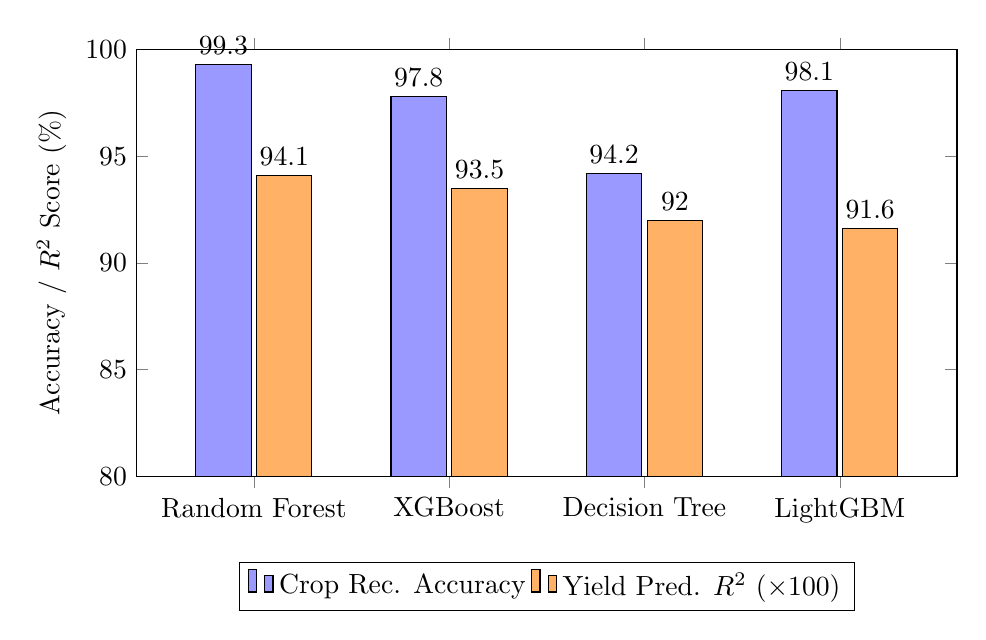
\begin{tikzpicture}
\begin{axis}[
    ybar,
    width=12cm,
    height=7cm,
    enlarge x limits=0.2,
    legend style={at={(0.5,-0.2)}, anchor=north, legend columns=-1},
    ylabel={Accuracy / $R^2$ Score (\%)},
    symbolic x coords={Random Forest, XGBoost, Decision Tree, LightGBM},
    xtick=data,
    nodes near coords,
    nodes near coords align={vertical},
    ymin=80, ymax=100,
    bar width=20pt,
]
% Crop Recommendation Accuracy (Percentage)
\addplot[fill=blue!40] coordinates {(Random Forest, 99.3) (XGBoost, 97.8) (Decision Tree, 94.2) (LightGBM, 98.1)};
% Yield Prediction R2 Score (Scaled to percentage for visualization)
\addplot[fill=orange!60] coordinates {(Random Forest, 94.1) (XGBoost, 93.5) (Decision Tree, 92.0) (LightGBM, 91.6)};

\legend{Crop Rec. Accuracy, Yield Pred. $R^2$ ($\times 100$)}
\end{axis}
\end{tikzpicture}
\caption{Comparative performance analysis of multiple machine learning models evaluated for the AgriDSS system.}
\end{figure}

\newpage

% ==============================================================================
% DIAGRAM 5: COMPONENT/CLASS DIAGRAM
% Useful for Chapter 3: Software Structure
% ==============================================================================
\section*{5. Software Component Architecture Diagram}

\begin{figure}[htbp]
\centering
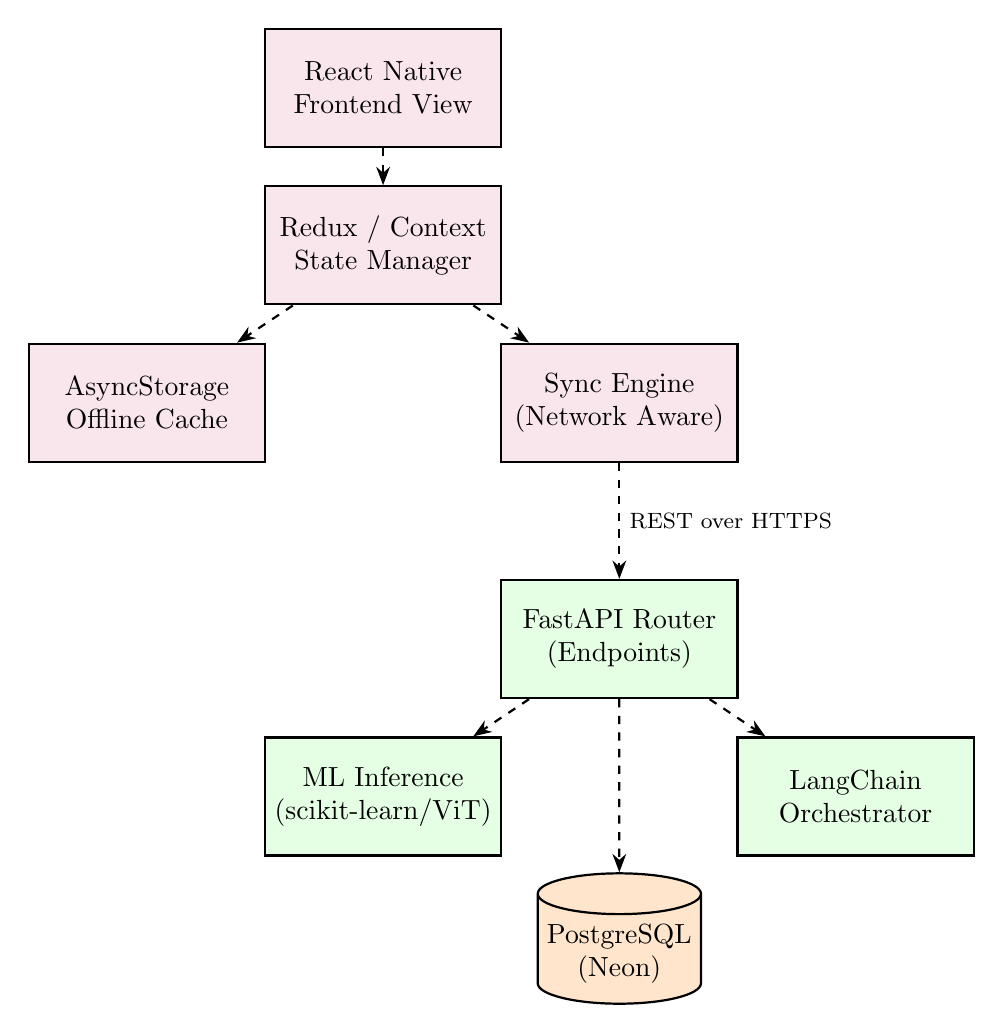
\begin{tikzpicture}[
  comp/.style={rectangle, draw, thick, fill=gray!10, minimum width=3cm, minimum height=1.5cm, align=center},
  db/.style={cylinder, draw, thick, fill=orange!20, aspect=0.25, minimum height=1.5cm, minimum width=2cm, align=center, shape border rotate=90},
  arr/.style={->, -{Stealth}, thick, dashed}
]

% UI Components
\node[comp, fill=purple!10] (ui) at (0,4) {React Native\\Frontend View};
\node[comp, fill=purple!10] (state) at (0,2) {Redux / Context\\State Manager};
\node[comp, fill=purple!10] (cache) at (-3,0) {AsyncStorage\\Offline Cache};
\node[comp, fill=purple!10] (sync) at (3,0) {Sync Engine\\(Network Aware)};

% Backend Components
\node[comp, fill=green!10] (api) at (3,-3) {FastAPI Router\\(Endpoints)};
\node[comp, fill=green!10] (ml) at (0,-5) {ML Inference\\(scikit-learn/ViT)};
\node[comp, fill=green!10] (llm) at (6,-5) {LangChain\\Orchestrator};

% Database
\node[db] (postgres) at (3,-7) {PostgreSQL\\(Neon)};

% Connections
\draw[arr] (ui) -- (state);
\draw[arr] (state) -- (cache);
\draw[arr] (state) -- (sync);
\draw[arr] (sync) -- node[right, font=\footnotesize] {REST over HTTPS} (api);
\draw[arr] (api) -- (ml);
\draw[arr] (api) -- (llm);
\draw[arr] (api) -- (postgres);

\end{tikzpicture}
\caption{Software Component Diagram detailing the separation of concerns between state management, ML inference, and persistence.}
\end{figure}

\vspace{1cm}

% ==============================================================================
% DIAGRAM 6: PIE CHART OF DISEASE DATASET DISTRIBUTION
% Useful for Chapter 4 or 5: Dataset descriptions
% (Requires \usepackage{pgf-pie})
% ==============================================================================
\section*{6. Dataset Distribution Pie Chart}

\begin{figure}[htbp]
\centering
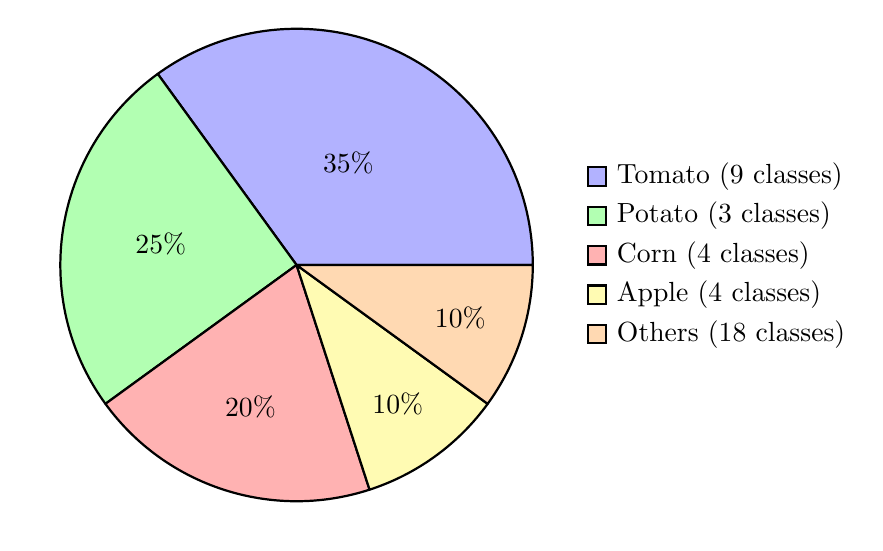
\begin{tikzpicture}
  \pie[
    color={blue!30, green!30, red!30, yellow!30, orange!30},
    text=legend,
    radius=3
  ]{
    35/Tomato (9 classes), 
    25/Potato (3 classes), 
    20/Corn (4 classes), 
    10/Apple (4 classes), 
    10/Others (18 classes)
  }
\end{tikzpicture}
\caption{Distribution of crop species in the 38-class fine-tuning dataset utilized for the Vision Transformer model.}
\end{figure}

\end{document}
